\chapter{Background}

\section{State of Art}

\section{OPC UA}
\subsection{Introduction}
In a proprietary system, connected devices may use different communication protocols. Software used to inspect and operate this system must be aware of all these protocols. 
This requires additional costs and time spent on creating and maintaining such a system. The complexity can be reduced by using the OPC UA standard for communication \cite{CPOpcTech}.

\subsection{Legacy OPC}
OPC is a data exchange standard for communication between multiple data sources. These sources may include factory devices, laboratory equipment, databases, and test system fixtures. A set of standard interfaces were defined by OPC Foundation to allow access to any device compatible with OPC \cite{whatopc}.

The first protocol is referred to as OPC Classic and it used Microsoft's COM(Component Object Model)/DCOM(Distributed Component Object Model) technology. 
COM/DCOM enabled communication between processes in multiple languages for Windows operating system. 
COM is an interface standard designed for software components and it allows systems to be built from different software vendors, that are designed to use this interface
COM is providing a communication interface layer, allowing both local and remote procedure calls between processes. 
Distributed COM (DCOM) is an extension of COM designed for distributed applications. DCOM allows components to communicate across the network \cite{COMDCOM, intrOPC}.

The OPC Classic specifications provided definitions for accessing data, alarms, events, and historical data \cite{OPCCLas}:
\begin{itemize}
  \item OPC Data Access (DA) - exchange of data which includes values, time and quality information in real time,
  \item OPC Historical Data Access (HDA) - reading, updating, and subscribing to historical data and events,
  \item and OPC Alarms and Events (A\&E) - receiving alarms and responding to them, reveiving events.
\end{itemize}

Because it relies on the Microsoft Windows platform, OPC Classic has some limitations like security issues or dependency on Windows \cite{whyOPC}.

{  
\color{red}
OPC Implementation? - jest to calkiem fajnie opisane w \cite{intrOPC}, ale nie wiem czy doda� bo mozliwe ze by�by to zbyt duzy offtop, bo uzywam opc ua.
}
\subsection{OPC UA}
In 2006 OPC Foundation released OPC Unified Architecture (UA) which is an improvement on OPC Classic. It brings together all the different specifications of OPC Classic into a single entry point with DA, A\&E with HDA of both.

\subsubsection{Communication impovements}
OPC UA is based on a cross-platform Service-Oriented Architecture (SOA). SOA is an improvement on the security and functionality that was in OPC Classic with Microsofts COM/DCOM technology.

OPC UA supports two protocols:
\begin{itemize}
  \item Binary protocol - requires minimal resources, easy passing through firewall
  \item Simple Object Access Protocol (SOAP) - uses HTTP/HTTPS ports
\end{itemize}

By using SOA and web services OPC UA became independent from Windows operating system. It means devices no longer had to be running Windows and OPC UA could be deployed on other operating systems, like Linux or Mac \cite{whyOPC}.

\subsubsection{Security imporovements} \label{sec-imporovements}
Security in OPC UA was greatly improved by switching from COM/DCOM. OPC Classic used security features from DCOM, which were complex and difficult. This caused common oversights in that department and disabled the security options altogether.

To secure data, OPC UA uses common web technologies as a security basis, which includes authentication and encryption features. Clients and servers use certificates to connect. OPC UA supports PKCS12 Public-Key Cryptography Standards to supply the X.509 private keys and certificate files containing public keys. 
There are three possible messaging modes between the server and client, wich are: None, Sign and Sign and Encrypt.
User also has the ability to enable Basic256 or Basic128Rsa15 security policy, which are bases for signing and encrypting the data \cite{whyOPC}.

\subsection{OPC UA Specification}
Specifications of OPC UA are split into parts, also known as IEC 62541 standards. The specifications parts are divided between core specifications, which establish the base for OPC UA, and access type specific elements, which specify information models. An overview showing these specifications is presented in the figure \ref{fig:opc-ua-spec}.

\begin{figure}[ht]
  \centering
  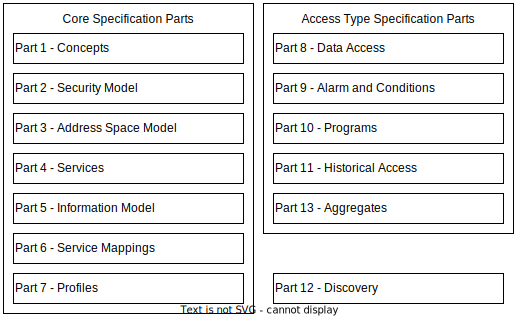
\includegraphics[width=0.7\linewidth]{figures02/OPC-ua-specification.pdf}
  \caption{OPC UA Specifications \cite{Damm2009OPCUA}}
  \label{fig:opc-ua-spec}
\end{figure}

\subsubsection{Core specification parts}
The concepts in part 1 provide an overview of OPC UA, and the security requirements and model are described in part 2. Further description of security part is in \ref{security}.

The specifications that are crucial to understanding how to model and access information are parts 3 and part 4. 

The Address Space Model in part 3 specifies the model used to define and expose information models, as well as to create an OPC UA address space. 

The possible relations between OPC UA client and server applications are represented in abstract UA Services in part 4. Client applications use Services to get information from the server. The services are not defined as a concrete representation of communication used by an application, but they define the information to be exchanged.

Part 6 explains how the UA Services are mapped to messages, how security methods are applied to them, and how the messages are wired. 

Part 5 contains the base information model, which is used to create information models that use OPC UA. This specification part defines:
\begin{itemize}
  \item The entry points into the address space that clients use to navigate through the instances and types of an OPC UA server
  \item The base types that serve as the foundation for the various type hierarchies
  \item The built-in but extensible types such as object types and data types
  \item The Server Object that provides capability and diagnostic information
\end{itemize}

The profiles in part 7 are used to define subsets of OPC UA features to implement by an UA application to provide interoperability for such subsets. Two levels of subsets are defined in the specification:
\begin{itemize}
  \item Conformance Units - first level, defines a small set of functionality that is used together and can be tested and verified
  \item Profiles - second level, list of conformance units
\end{itemize}

\subsubsection{Access type specification parts}

Part 8 includes the Data Access information model, which defines the representation and usage of automation data and specific characteristics.
Process alarm and condition monitoring are specified in the Alarms and Conditions information model defined in part 9.
Part 10 contains the Programs information model that defines a base state machine. 
The Historical Access information model describes the usage of history access Services and the presentation of information in part 11.
In part 13 the Aggregates specifies the computation of aggregated values from data samples.

\subsubsection{Discovery part}

The Discovery specifies how to discover servers in the network and how to get the necessary information needed for connection from a client in part 12 \cite{Damm2009OPCUA}. Additional descriptions are provided in \ref{data-acc}

\subsubsection{Information modeling} \label{inf-modeling}
The meta model of OPC UA is defined in part 3 of the specification. The base component of the meta model is nodes. For specializing the base node class, several node classes are defined \ref*{fig:opc-ua-base}, like variables, objects, etc. Nodes have a set of attributes for each, depending on the class. Some attributes are required, while others are optional. Each node class, for example, requires a "NodeId" that uniquely identifies the node, but the "Description" is optional \cite{Leitner2006OPCU}.

\begin{figure}[ht]
  \centering
  \includegraphics[width=0.8\linewidth]{figures02/opc-meta-model.pdf}
  \caption{OPC UA meta model \cite{Leitner2006OPCU}}
  \label{fig:opc-ua-base}
\end{figure}

The base principles of data modeling in OPC UA are \cite{Damm2009OPCUA, PAUKER2016321}:
\begin{itemize}
  \item Object-oriented techniques with type hierarchies and inheritance,
  \item Type information is available and can be accessed similarly to an instance,
  \item A fully mesh network of nodes allows information to be connected in a variety of ways,
  \item Type hierarchies, as well as reference types between nodes, are extensible,
  \item No modeling limits to allow for proper information model design,
  \item OPC UA information modeling is always done on the server.
\end{itemize}

\subsection{OPC UA software layers}
OPC UA uses the client-server concept for communication. The UA server application exposes its information to other applications and the UA client is an application that consumes that information. An application might serve both as a UA server and client.

OPC UA is most often created from three software layers, as shown in \ref{fig:opc-ua-layers}. There is presented that the whole software stack can be implemented in Java, C/C++, or .NET, but it is also possible to implement it in javascript, as in this thesis.

\begin{figure}[ht]
  \centering
  \includegraphics[width=0.7\linewidth]{figures02/opc-software-layers.pdf}
  \caption{OPC UA software layers \cite{Damm2009OPCUA}}
  \label{fig:opc-ua-layers}
\end{figure}

OPC UA Application is a system that exposes or consumes information through OPC UA. OPC UA client or server SDK contains OPC UA functionalities, and UA Stacks implement communication channels \cite{Damm2009OPCUA}.


\section{OPC UA comparison to other communication protocols}
\subsection{MQTT}
MQTT (Message Queue Telemetry Transport) is a lightweight message protocol based on a subscription-publishing model in which publishers send messages to a server, which then forwards them to subscribers, avoiding point-to-point connections between subscribers and publishers. This eliminates the need for subscribers to know who provides the information to which they have subscribed. MQTT was created with low-resource devices, low-bandwidth networks, and high latency in mind \cite{MQTTvsOPC-UA}.

\subsection{MTConnect}
The MTConnect standard (ANSI/MTC1.4-2018) provides a semantic vocabulary for manufacturing equipment that allows it to provide structured, contextualized data in any format. Developers and integrators can concentrate on interesting, productive manufacturing applications rather than translation with homogeneous data. Machine tools, industrial equipment, sensors and sensor controllers, and other factory hardware are all data sources \cite{MTConnect}.
% TODO zmieni� troch� imo

\subsection{Protocol elements}

MTConnect uses client-agent concept for communication. Path of communication of components and devices with agent is proprietary. 
The agent-client interface is specified as a RESTful interface based on HTTP. This type of communication allows it to be stateless. This means that the server does not need to have session managemement, which provides simplicity. However, there is no user authentication during setup. MTConnect have specified only the GET method of HTTP request methods. It is used to get information without any side effects \cite{Michaloski2009QuantifyingTP}, so data transport is made very simple. The application data of the agent are transferred in XML format \cite{MQTTvsOPC-UA}.  

MQTT uses client-server concept for communication. The protocol runs over TCP/IP, or other other network protocols providing ordered, lossless, bi-directional connectivity. Message payloads can be sent in any format. MQTT uses publish/subscribe message pattern, which allows for one-to-many message distribution and application decoupling. The client can both subscribe to topics and publish messages. 
The protocol supports sending messages with quality of service with three levels:   
\begin{itemize}
  \item "At most once" - no quality of service. Message is sent only once, so if client is not available the message will be lost
  \item "At least once" - message will be resent until it is received at least once. Duplication of messages may occur
  \item "Exactly once" - message is assured to arrive exactly once \cite{MQTT50, opc-vs-mtconnect}.
\end{itemize}

OPC UA client-server communication runs over TCP/IP, SOAP/HTTP and HTTPS. SOAP is an XML-based protocol that allows for HTTP-based message exchanges that follow the request and response pattern. The OPC UA messages are sent over WS (Web Service) Secure Conversation and SOAP using OPC UA Binary Encoding. Base64 is less effecient compared to binary coding, but it is more efficitent that than XML used by MTConnect. 
The WS Secure Conversation specification is part of the web service specification series, which provides a collection of specifications for SOAP/WSDL-based services. 
HTTPS allows OPC UA Binary and XML to be transferred over a secure SSL/TLS connection.

\subsection{Data models}

MTConnect has very detailed data model that is thoroughly specified in XML schemas. It uses a single catalog of terminology and phrases to make it brief and straightforward. The rigidity of this process, however, is a disadvantage. Only a change or extension of the standard will allow the model to be extended or modified \cite{opc-vs-mtconnect}.

MQTT packet structure is consisting of always present fixed header, not always present variable header, and payload \cite{MQTTprot}. There is no data model for payload, therefore messages can be transmitted in any format, including JSON, XML, encrypted binary, and Base64. This provides the protocol a lot of flexibility, but it also means that the client receiving the messages needs to be able to analyze type of load that is incoming \cite{MQTTvsOPC-UA}.

OPC UA uses information model defined in part 3 of it's specification, described in \ref{inf-modeling}. The information model allows changes like adding and deleting nodes during runtime of the server, which is an advantage when compared to MTConnect, but it still is an effort to implement this data model \cite{opc-vs-mtconnect}. MQTT gives a lot more freedom when modeling the data model.

\subsection{Data access and discovery} \label{data-acc}

It is recommended to use LDAP server (Lightweight Directory Access Protocol) and thus a standard method to detect MTConnect-enabled devices. The agents log in all devices connected to them. To read out the structure of the components and data items, MTConnect defines the call type "probe", which allows a kind of browsing of the device representation. Other call types are used to read immediate values, such as events and states, and to read different histories. An agent stores the acquired data in a ring buffer, which may result in data loss due to overwriting. The client-side application is in charge of the timely reading \cite{opc-vs-mtconnect}. 

MQTT is designed to be lightweight and energy efficient, so it does not have implemented any mechanism of search of the topic nor the broker where messages are published. Client application has to have knowledge of broker and message topics beforehand \cite{MQTTvsOPC-UA}. 

OPC UA offers a Discovery Endpoint, which can be used by clients to retrieve the configuration of the server. The LDS (Local Discovery Server) is used when multiple devices are hosting OPC UA servers. These servers register their endponts to the LDS. OPC UA servers on a subnet can be also discovered through multicast DNS. OPC UA defines also a GDS (Global Directory Service) as a central server with methods for directory managemement. If OPC UA servers register at this service, then clients can browse lists of these servers \cite{opc-vs-mtconnect}.

\subsection{Security} \label{security}

With MTConnect security is treated with lower priority. It is recommended that implementations include encryption of data transport and storage by standard methods such as SSL/TLS for transport and AES of RSA for storing \cite{opc-vs-mtconnect}.

MQTT allows implementers a choice of network, privacy, authentication and authorization technologies. It is on implementer responsibility to include security features as part of the design. In hostile communication environments it is recommended to use methods like TLS and provide mechanisms for authentication of users, authorization of access, integrity and privacy of MQTT Control Packets and application data within \cite{MQTT50}.

In OPC UA security is an integral part of the specification, and it is described in part 2 of this specification. Security functions are defined at different levels, as a mandatory part of the protocol. The features include authenticity, authorisation, integrity and confidentiality. As described ealier in \ref{sec-imporovements}, applications are expected to exchange certificates for the identification. Individual data elements can have granular access rights applied to them. Transfer of data is encrypted with SSL/TLS, the WS Secure Conversation, and the particular UA Secure Conversation \cite{opc-vs-mtconnect}.


\section{Abstraction layers}
\subsection{Introduction}
Systems created currently are constructed using numerous abstraction layers. Each layer is defining an inteface that hides details of implementation for its functionality. Programs that are built on top of each layer can be used and understood using only its inteface, so it's not necessary to know the layer implementation.
\subsection{Specification}
Important aspect of an abstraction layer is its specification. A specification should capture the functionality of the implementation as well as the assuptions about other layer context. However, abstraction layers are not commonly specified and verified.
\subsection{Issues}
{
  \color{red}
  Write something about issues when creating abstraction layers\\
  
  sources: \\
  Deep Specifications and Certified Abstraction Layers \\
  http://flint.cs.yale.edu/flint/publications/dscal.pdf\\
  
  Separation Logic: A Logic for Shared Mutable Data Structures \\
  https://sci-hub.se/10.1109/LICS.2002.1029817\\
  https://ieeexplore.ieee.org/document/1029817\\
  
  Theories of Programming Languages\\
  John C. Reynolds\\
  
  Clean code\\
  str 36, 93, 290\\
}

\section{C4 model}
The C4 model is a graphical notation technique for representing software system architecture\cite{Richards2020FundamentalsOS, EnriquezReneSalazarAlbertoArchitecture2018}. 
It is built on a structural decomposition of a system into containers and components, and it depends on existing modeling approaches such as the Unified Modeling Language (UML) or Entity Relation Diagrams (ERD) for a more precise decomposition of the architectural building blocks. 
It also was developed to address UML's shortcomings and improve its approach \cite{Richards2020FundamentalsOS}.

\subsection{Abstractions}
The C4 model is an "abstraction-first" approach to diagramming software architecture, based upon abstractions that illustrate how software architects and developers think about and build software \cite{C4Model}.

Model created using C4 is composed of a set of hierarchical diagrams, that can be used to describe software at different levels of detail \cite{C4ModelSimon, C4Model}:
\begin{itemize}
  \item System Context diagram - shows the overall software information and how the software system in scope would fit into the world around it,
  \item Container diagram - more detailed diagram of the software system, showing containers that together create that software system. Containers might be applications, data stores, microservices, etc. The key part of this level is technology decisions on what would be used to develop each part.
  \item Component diagram - a diagram showing details and components of the selected container. Components should map to real abstractions, e.g. a grouping of code in the codebase.
  \item Code diagram - diagram of the selected component, showing how this component is implemented. It can be created using, for example, a UML class diagram. This level is not often used by software architects and developers because it is too much detailed to be practical.
\end{itemize}

An overview of these levels is illustrated in \ref{fig:c4-overview}

% TODO powrzuca� lepiej widoczne zdj�cia
\begin{figure}[ht]
  \centering
  \includegraphics[width=1\linewidth]{figures02/c4-overview.png}
  \caption{C4 model \cite{C4Model}}
  \label{fig:c4-overview}
\end{figure}

\subsection{Notation}
There is no particular nota

